\documentclass{beamer}
\usepackage[T1]{fontenc}
\usepackage[utf8x]{inputenc} 
\usepackage[esperanto]{babel}
%\usepackage{umbcboxes}

\title{Trelliĝu}
\subtitle{ang. ,,get trelled''}
\author{Tomasz Szymula}
\institute[PEJ]{
\includegraphics[scale=0.3]{bildoj/pej}}

\date[IJS 2014]{Internacia Junulara Semajno, 2014 Horány}
\subject{}

\usetheme{Warsaw}
\usecolortheme{beaver}

\AtBeginSubsection[]
{
  \begin{frame}
    \frametitle{Plano}
    \tableofcontents[currentsection]
  \end{frame}
}

\begin{document}
  \frame{\titlepage}
  
\section{Pri kio temas}
\subsection{Kia problemo estas?}

%%%>>>>>>>>>>>>>>>>>>>>>>>>>>>>>>>>>>>>>>>>>>>>>>>>>>>>>>>>>>>>>>>>>>>>>>>>>>>>>>>>>>>>>>>>>>>>>>
  \begin{frame}
    \frametitle{Komenco}
    \framesubtitle{Vi havas 20 novajn mesaĝojn.}
    
	\begin{center}
    	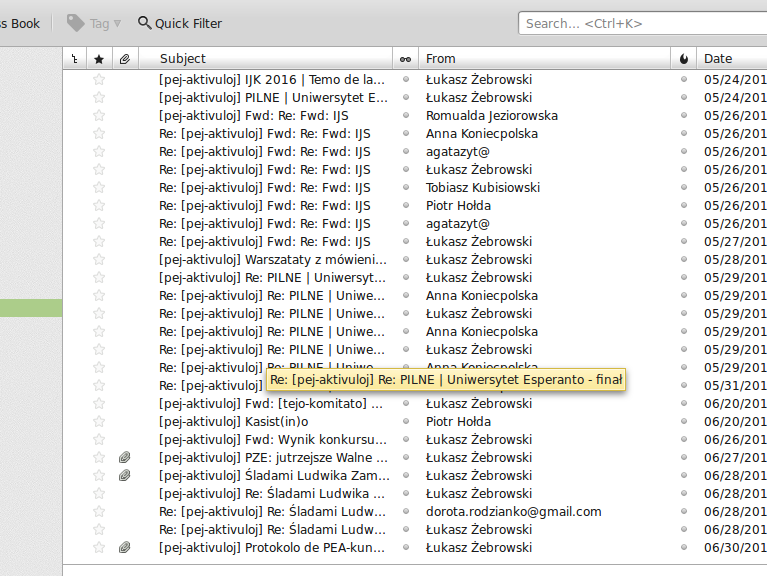
\includegraphics[scale=0.3]{ekranoj/retposhto}
	\end{center}
  \end{frame}
%%%<<<<<<<<<<<<<<<<<<<<<<<<<<<<<<<<<<<<<<<<<<<<<<<<<<<<<<<<<<<<<<<<<<<<<<<<<<<<<<<<<<<<<<<<<<<<<<
 

%%%>>>>>>>>>>>>>>>>>>>>>>>>>>>>>>>>>>>>>>>>>>>>>>>>>>>>>>>>>>>>>>>>>>>>>>>>>>>>>>>>>>>>>>>>>>>>>>
  \begin{frame}
    \frametitle{Retpoŝto}
    \framesubtitle{Ĉu vi ŝatas ĝin uzi por esperantaj projektoj?}
    \begin{itemize}
    	\item Kiom da retadresoj vi uzas?
    	\item Kiom da esperanto-rilataj (nepersonaj = malinteresaj) mesaĝoj vi ricevas semajne?
    	\item Kiom da el ili rilatas rekte al vi?
    	\item Ĉu vi ĉiam (iam ajn?) tuj recivinte la mesaĝon plenumas peton/taskon au prokrastetas?
    \end{itemize}
  \end{frame}
%%%<<<<<<<<<<<<<<<<<<<<<<<<<<<<<<<<<<<<<<<<<<<<<<<<<<<<<<<<<<<<<<<<<<<<<<<<<<<<<<<<<<<<<<<<<<<<<<
   
   
\subsection{Kiel solvi?}
   
%%%>>>>>>>>>>>>>>>>>>>>>>>>>>>>>>>>>>>>>>>>>>>>>>>>>>>>>>>>>>>>>>>>>>>>>>>>>>>>>>>>>>>>>>>>>>>>>>    
  \begin{frame}
    \frametitle{Taskolistoj?}

	\begin{block}{Ekzemplo}
    	\begin{center}
    	
\includegraphics[scale=0.5]{meme/to_do_list}
    	\end{center}
	\end{block}
    
    \begin{itemize}
    	\item Kiel tio helpas?
    	\item Ĉu vi ilin uzas por organizi sian ĉiutagan laboron?
    \end{itemize}
        
  \end{frame}    
%%%<<<<<<<<<<<<<<<<<<<<<<<<<<<<<<<<<<<<<<<<<<<<<<<<<<<<<<<<<<<<<<<<<<<<<<<<<<<<<<<<<<<<<<<<<<<<<<


   
%%%>>>>>>>>>>>>>>>>>>>>>>>>>>>>>>>>>>>>>>>>>>>>>>>>>>>>>>>>>>>>>>>>>>>>>>>>>>>>>>>>>>>>>>>>>>>>>>
  \begin{frame}
    \frametitle{Taskolistoj!}
    %http://www.learningcommons.uoguelph.ca/guides/time_management/html/making_task_list.html
    Ne forgesu, ke:
    \begin{itemize}
    	\item Tio helpas memori eĉ pri flankaj taskoj.
     	\item Oni povas taksi la prioritatojn = sukcesi ĝis limdatoj
        \item Malpli da prokrastado, ĉar vi havos realecan imagon kiom da laboro vere farendas.      
    \end{itemize}
  \end{frame}      
%%%<<<<<<<<<<<<<<<<<<<<<<<<<<<<<<<<<<<<<<<<<<<<<<<<<<<<<<<<<<<<<<<<<<<<<<<<<<<<<<<<<<<<<<<<<<<<<<


\subsection{Trello}
   
%%%>>>>>>>>>>>>>>>>>>>>>>>>>>>>>>>>>>>>>>>>>>>>>>>>>>>>>>>>>>>>>>>>>>>>>>>>>>>>>>>>>>>>>>>>>>>>>>
  \begin{frame}
    \frametitle{Mia propono: Trello.com}
    
    
  \end{frame}
%%%<<<<<<<<<<<<<<<<<<<<<<<<<<<<<<<<<<<<<<<<<<<<<<<<<<<<<<<<<<<<<<<<<<<<<<<<<<<<<<<<<<<<<<<<<<<<<<
  
%%%>>>>>>>>>>>>>>>>>>>>>>>>>>>>>>>>>>>>>>>>>>>>>>>>>>>>>>>>>>>>>>>>>>>>>>>>>>>>>>>>>>>>>>>>>>>>>>
  \begin{frame}
    \frametitle{Kial -- la bildoj sinesprimas.}
    \framesubtitle{Elektu!}
    
	\begin{columns}
    \column{0.5\textwidth}
	    \begin{center}
    		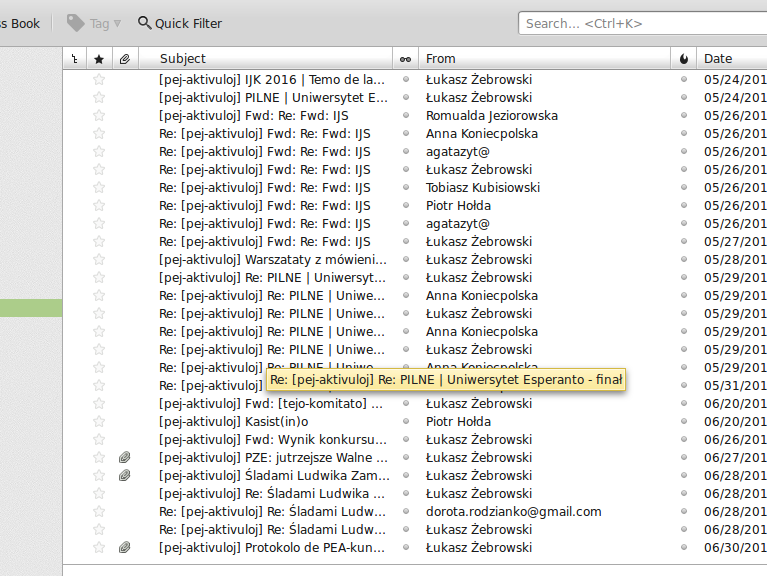
\includegraphics[scale=0.2]{ekranoj/retposhto}
    	\end{center}
	\column{0.5\textwidth}
    	\begin{center}
    	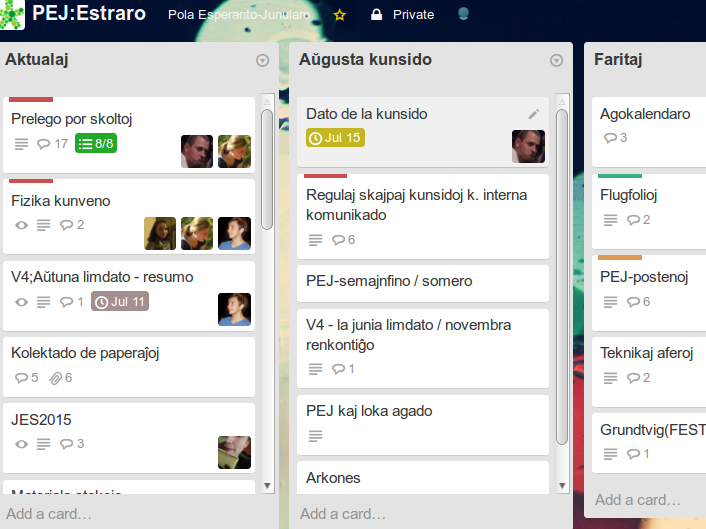
\includegraphics[scale=0.22]{ekranoj/trello-bonas-estraro}
    	\end{center}

	\end{columns}
  \end{frame}
%%%<<<<<<<<<<<<<<<<<<<<<<<<<<<<<<<<<<<<<<<<<<<<<<<<<<<<<<<<<<<<<<<<<<<<<<<<<<<<<<<<<<<<<<<<<<<<<<



%%%>>>>>>>>>>>>>>>>>>>>>>>>>>>>>>>>>>>>>>>>>>>>>>>>>>>>>>>>>>>>>>>>>>>>>>>>>>>>>>>>>>>>>>>>>>>>>>
  \begin{frame}
    \frametitle{Trello - kiu ĝin uzas?}
    
    
  \end{frame}
%%%<<<<<<<<<<<<<<<<<<<<<<<<<<<<<<<<<<<<<<<<<<<<<<<<<<<<<<<<<<<<<<<<<<<<<<<<<<<<<<<<<<<<<<<<<<<<<<
  
  

%%%>>>>>>>>>>>>>>>>>>>>>>>>>>>>>>>>>>>>>>>>>>>>>>>>>>>>>>>>>>>>>>>>>>>>>>>>>>>>>>>>>>>>>>>>>>>>>>
  \begin{frame}
    \frametitle{Ne nur Trello}
    
  \end{frame}
%%%<<<<<<<<<<<<<<<<<<<<<<<<<<<<<<<<<<<<<<<<<<<<<<<<<<<<<<<<<<<<<<<<<<<<<<<<<<<<<<<<<<<<<<<<<<<<<<


%%%%%%%%%%%%%%%%%%%%%%%%%%%%%%%%%%%%%%%%%%%%%%%%%%%%%%%%%%%%%%%%%%%%%%%%%%%%%%%%%%%%%%%%%%%%%%%%%
%%%%%%%%%%%%%%%%%%%%%%%%%%%%%%%%%%%%%%%%%%%%%%%%%%%%%%%%%%%%%%%%%%%%%%%%%%%%%%%%%%%%%%%%%%%%%%%%%
%%%%%%%%%%%%%%%%%%%%%%%%%%%%%%%%%%%%%%%%%%%%%%%%%%%%%%%%%%%%%%%%%%%%%%%%%%%%%%%%%%%%%%%%%%%%%%%%%

\section{Praktika enkonduko}
\subsection{Uzantkontoj}
%%%>>>>>>>>>>>>>>>>>>>>>>>>>>>>>>>>>>>>>>>>>>>>>>>>>>>>>>>>>>>>>>>>>>>>>>>>>>>>>>>>>>>>>>>>>>>>>>
  \begin{frame}
    \frametitle{Ensalutu en trellon}

	Uzu sian propran konton aŭ uzu unu de la subaj:

%	\begin{tabular}{ | c | c | }
%	\hline                       
%		anaso_trejnanto gmail.com & 2anasoj \\
%		alaudo_trejnanto gmail.com & 2alaudoj \\
%		najtingalo_trejnanto gmail.com & 2najgingaloj \\
%		kolombo_trejnanto gmail.com & 2kolomboj\\
%	\hline  
%	\end{tabular}

\end{frame}
%%%<<<<<<<<<<<<<<<<<<<<<<<<<<<<<<<<<<<<<<<<<<<<<<<<<<<<<<<<<<<<<<<<<<<<<<<<<<<<<<<<<<<<<<<<<<<<<<


%%%>>>>>>>>>>>>>>>>>>>>>>>>>>>>>>>>>>>>>>>>>>>>>>>>>>>>>>>>>>>>>>>>>>>>>>>>>>>>>>>>>>>>>>>>>>>>>>
  \begin{frame}
    \frametitle{Bongusta horloĝo!}
    %\includegraphics{ mazi manĝas la horloĝon :-)}
  \end{frame}
%%%<<<<<<<<<<<<<<<<<<<<<<<<<<<<<<<<<<<<<<<<<<<<<<<<<<<<<<<<<<<<<<<<<<<<<<<<<<<<<<<<<<<<<<<<<<<<<<

\subsection{Para klakado}
%%%>>>>>>>>>>>>>>>>>>>>>>>>>>>>>>>>>>>>>>>>>>>>>>>>>>>>>>>>>>>>>>>>>>>>>>>>>>>>>>>>>>>>>>>>>>>>>>
  \begin{frame}
    \frametitle{Pariĝu!}
    Kaj decidu kiu unue estos kunordiganto (poste la roloj interŝanĝiĝos).
  \end{frame}
%%%<<<<<<<<<<<<<<<<<<<<<<<<<<<<<<<<<<<<<<<<<<<<<<<<<<<<<<<<<<<<<<<<<<<<<<<<<<<<<<<<<<<<<<<<<<<<<<

%%%>>>>>>>>>>>>>>>>>>>>>>>>>>>>>>>>>>>>>>>>>>>>>>>>>>>>>>>>>>>>>>>>>>>>>>>>>>>>>>>>>>>>>>>>>>>>>>
  \begin{frame}
    \frametitle{Kreu la tabulon por la matenmanĝa projekto!}
  \end{frame}
%%%<<<<<<<<<<<<<<<<<<<<<<<<<<<<<<<<<<<<<<<<<<<<<<<<<<<<<<<<<<<<<<<<<<<<<<<<<<<<<<<<<<<<<<<<<<<<<<

%%%>>>>>>>>>>>>>>>>>>>>>>>>>>>>>>>>>>>>>>>>>>>>>>>>>>>>>>>>>>>>>>>>>>>>>>>>>>>>>>>>>>>>>>>>>>>>>>
  \begin{frame}
    \frametitle{Ekzerco}
    Kunordiganto:
        Kreu karton "manĝajho"
        komponu la liston de la bazaj bezonataj artikoloj: pano, smirajho
    Manĝorespondeculo
        aldonu buteron al la listo
        demandu la kunordiganton kiom da konfituraĵo meti sur la panon (demetu sin de la karto kaj metu la kunordiganton)
    Kunordiganto:
        respondu (demetu sin kaj remetu manĝrespondeculon)
    Manĝrespondeculo:
        eklaboru! se vi havas pliajn demandojn ("kie estas pano?") ktp
  \end{frame}
%%%<<<<<<<<<<<<<<<<<<<<<<<<<<<<<<<<<<<<<<<<<<<<<<<<<<<<<<<<<<<<<<<<<<<<<<<<<<<<<<<<<<<<<<<<<<<<<<


%%%>>>>>>>>>>>>>>>>>>>>>>>>>>>>>>>>>>>>>>>>>>>>>>>>>>>>>>>>>>>>>>>>>>>>>>>>>>>>>>>>>>>>>>>>>>>>>>
  \begin{frame}
    \frametitle{Intershanĝu la rolojn!}
    Kunordiganto iĝas teorespondeculo
    Manĝrespondeculo iĝas kunordiganto
  \end{frame}
%%%<<<<<<<<<<<<<<<<<<<<<<<<<<<<<<<<<<<<<<<<<<<<<<<<<<<<<<<<<<<<<<<<<<<<<<<<<<<<<<<<<<<<<<<<<<<<<<

%%%>>>>>>>>>>>>>>>>>>>>>>>>>>>>>>>>>>>>>>>>>>>>>>>>>>>>>>>>>>>>>>>>>>>>>>>>>>>>>>>>>>>>>>>>>>>>>>
  \begin{frame}
    \frametitle{Kunordiganto: kreu la tabulon por la teoumada projekto!}
    
  \end{frame}
%%%<<<<<<<<<<<<<<<<<<<<<<<<<<<<<<<<<<<<<<<<<<<<<<<<<<<<<<<<<<<<<<<<<<<<<<<<<<<<<<<<<<<<<<<<<<<<<<

%%%>>>>>>>>>>>>>>>>>>>>>>>>>>>>>>>>>>>>>>>>>>>>>>>>>>>>>>>>>>>>>>>>>>>>>>>>>>>>>>>>>>>>>>>>>>>>>>
  \begin{frame}
    \frametitle{Ekzerco!}

    Inversa scenario pri teo
  \end{frame}
%%%<<<<<<<<<<<<<<<<<<<<<<<<<<<<<<<<<<<<<<<<<<<<<<<<<<<<<<<<<<<<<<<<<<<<<<<<<<<<<<<<<<<<<<<<<<<<<<

\section{Teorio}

\subsection{Kartoj}
%%%>>>>>>>>>>>>>>>>>>>>>>>>>>>>>>>>>>>>>>>>>>>>>>>>>>>>>>>>>>>>>>>>>>>>>>>>>>>>>>>>>>>>>>>>>>>>>>
  \begin{frame}
    \frametitle{Vi kaj viaj kartoj}

	\begin{block}{Ĝenerala regulo}
		Se vi estas sur iu karto, vi \textbf{devas fari ion konkretan}
	\end{block}
  \end{frame}
%%%<<<<<<<<<<<<<<<<<<<<<<<<<<<<<<<<<<<<<<<<<<<<<<<<<<<<<<<<<<<<<<<<<<<<<<<<<<<<<<<<<<<<<<<<<<<<<<


\subsection{Sciigoj}
%%%>>>>>>>>>>>>>>>>>>>>>>>>>>>>>>>>>>>>>>>>>>>>>>>>>>>>>>>>>>>>>>>>>>>>>>>>>>>>>>>>>>>>>>>>>>>>>>
  \begin{frame}
    \frametitle{Kiam vi volas ricevi informojn?}
	\framesubtitle{Ĝeneralaj reguloj}
	\begin{block}{I}
		Kiam iu afero rilatas al vi, vi volas esti informata.
	\end{block}
	\begin{block}{II}
		Kiam afero ne rilatas al vi, vi ne volas aŭdi pri ĝi.
	\end{block}
	\begin{block}{III}
		Tamen en libera tempo estus bone havi eblecon trarigardi, kio okazas.
	\end{block}
	
  \end{frame}
%%%<<<<<<<<<<<<<<<<<<<<<<<<<<<<<<<<<<<<<<<<<<<<<<<<<<<<<<<<<<<<<<<<<<<<<<<<<<<<<<<<<<<<<<<<<<<<<<


%%%>>>>>>>>>>>>>>>>>>>>>>>>>>>>>>>>>>>>>>>>>>>>>>>>>>>>>>>>>>>>>>>>>>>>>>>>>>>>>>>>>>>>>>>>>>>>>>
  \begin{frame}
    \frametitle{Kio estas sciigo en Trello?}

	\begin{enumerate}
		\item Sendita retmesaĝo (unu sciigo=unu mesaĝo aŭ kelkaj ĝisdatigoj en unu mesaĝo - \alert{agordigeblas} )
		\item Novaĵoj ĉe trello.com
		\item Android/iPhone
		\item "desktop" (??)
	\end{enumerate}
  \end{frame}
%%%<<<<<<<<<<<<<<<<<<<<<<<<<<<<<<<<<<<<<<<<<<<<<<<<<<<<<<<<<<<<<<<<<<<<<<<<<<<<<<<<<<<<<<<<<<<<<<



%%%>>>>>>>>>>>>>>>>>>>>>>>>>>>>>>>>>>>>>>>>>>>>>>>>>>>>>>>>>>>>>>>>>>>>>>>>>>>>>>>>>>>>>>>>>>>>>>
  \begin{frame}
    \frametitle{Agordoj de sciigoj}

  \end{frame}
%%%<<<<<<<<<<<<<<<<<<<<<<<<<<<<<<<<<<<<<<<<<<<<<<<<<<<<<<<<<<<<<<<<<<<<<<<<<<<<<<<<<<<<<<<<<<<<<<


%%%>>>>>>>>>>>>>>>>>>>>>>>>>>>>>>>>>>>>>>>>>>>>>>>>>>>>>>>>>>>>>>>>>>>>>>>>>>>>>>>>>>>>>>>>>>>>>>
  \begin{frame}
    \frametitle{Abonu/malabonu tabulon/karton}

	\begin{columns}
    \column{0.5\textwidth}
	    \begin{block}{Karto}
	     
    	\end{block}
	\column{0.5\textwidth}
    	\begin{block}{Tabulo}
    	
    	\end{block}

	\end{columns}
  \end{frame}
%%%<<<<<<<<<<<<<<<<<<<<<<<<<<<<<<<<<<<<<<<<<<<<<<<<<<<<<<<<<<<<<<<<<<<<<<<<<<<<<<<<<<<<<<<<<<<<<<



%%%>>>>>>>>>>>>>>>>>>>>>>>>>>>>>>>>>>>>>>>>>>>>>>>>>>>>>>>>>>>>>>>>>>>>>>>>>>>>>>>>>>>>>>>>>>>>>>
  \begin{frame}
    \frametitle{Ĉiu projekto bezonas sian kunordiganton}

	\begin{block}{Praktika kaj efika difino}
		Kunordiganto de la projekto estas tiu, kiu devus honti, se la projekto malsukcesas. Pro tio liŝi zorgu, ke tio ne okazu.
	\end{block}
	    
  \end{frame}
%%%<<<<<<<<<<<<<<<<<<<<<<<<<<<<<<<<<<<<<<<<<<<<<<<<<<<<<<<<<<<<<<<<<<<<<<<<<<<<<<<<<<<<<<<<<<<<<<


%%%>>>>>>>>>>>>>>>>>>>>>>>>>>>>>>>>>>>>>>>>>>>>>>>>>>>>>>>>>>>>>>>>>>>>>>>>>>>>>>>>>>>>>>>>>>>>>>
  \begin{frame}
    \frametitle{Prezidanto?}
    
    Malrekomendindas, ke 
    
  \end{frame}
%%%<<<<<<<<<<<<<<<<<<<<<<<<<<<<<<<<<<<<<<<<<<<<<<<<<<<<<<<<<<<<<<<<<<<<<<<<<<<<<<<<<<<<<<<<<<<<<<
  

%%%>>>>>>>>>>>>>>>>>>>>>>>>>>>>>>>>>>>>>>>>>>>>>>>>>>>>>>>>>>>>>>>>>>>>>>>>>>>>>>>>>>>>>>>>>>>>>>
  \begin{frame}
    \frametitle{Fotoj gravas}

  \end{frame}
%%%<<<<<<<<<<<<<<<<<<<<<<<<<<<<<<<<<<<<<<<<<<<<<<<<<<<<<<<<<<<<<<<<<<<<<<<<<<<<<<<<<<<<<<<<<<<<<<


%%%>>>>>>>>>>>>>>>>>>>>>>>>>>>>>>>>>>>>>>>>>>>>>>>>>>>>>>>>>>>>>>>>>>>>>>>>>>>>>>>>>>>>>>>>>>>>>>
  \begin{frame}
    \frametitle{"Allow org members to join"}

    Eble metu tiun ĉi ĉe kreado de la tabulo...
  \end{frame}
%%%<<<<<<<<<<<<<<<<<<<<<<<<<<<<<<<<<<<<<<<<<<<<<<<<<<<<<<<<<<<<<<<<<<<<<<<<<<<<<<<<<<<<<<<<<<<<<<


%%%>>>>>>>>>>>>>>>>>>>>>>>>>>>>>>>>>>>>>>>>>>>>>>>>>>>>>>>>>>>>>>>>>>>>>>>>>>>>>>>>>>>>>>>>>>>>>>
  \begin{frame}
    \frametitle{"periodically send ĝisdatiĝoj"}

  \end{frame}
%%%<<<<<<<<<<<<<<<<<<<<<<<<<<<<<<<<<<<<<<<<<<<<<<<<<<<<<<<<<<<<<<<<<<<<<<<<<<<<<<<<<<<<<<<<<<<<<<


%%%>>>>>>>>>>>>>>>>>>>>>>>>>>>>>>>>>>>>>>>>>>>>>>>>>>>>>>>>>>>>>>>>>>>>>>>>>>>>>>>>>>>>>>>>>>>>>>
  \begin{frame}
    \frametitle{"Fulmklavoj"}

  \end{frame}
%%%<<<<<<<<<<<<<<<<<<<<<<<<<<<<<<<<<<<<<<<<<<<<<<<<<<<<<<<<<<<<<<<<<<<<<<<<<<<<<<<<<<<<<<<<<<<<<<


%%%>>>>>>>>>>>>>>>>>>>>>>>>>>>>>>>>>>>>>>>>>>>>>>>>>>>>>>>>>>>>>>>>>>>>>>>>>>>>>>>>>>>>>>>>>>>>>>
  \begin{frame}
    \frametitle{Etiketoj}

  \end{frame}
%%%<<<<<<<<<<<<<<<<<<<<<<<<<<<<<<<<<<<<<<<<<<<<<<<<<<<<<<<<<<<<<<<<<<<<<<<<<<<<<<<<<<<<<<<<<<<<<<


\subsection{Ekster esperantaj ekzemploj}

%%%>>>>>>>>>>>>>>>>>>>>>>>>>>>>>>>>>>>>>>>>>>>>>>>>>>>>>>>>>>>>>>>>>>>>>>>>>>>>>>>>>>>>>>>>>>>>>>
  \begin{frame}
    \frametitle{???}

  \end{frame}
%%%<<<<<<<<<<<<<<<<<<<<<<<<<<<<<<<<<<<<<<<<<<<<<<<<<<<<<<<<<<<<<<<<<<<<<<<<<<<<<<<<<<<<<<<<<<<<<<

\subsection{Ekzemploj}

%%%>>>>>>>>>>>>>>>>>>>>>>>>>>>>>>>>>>>>>>>>>>>>>>>>>>>>>>>>>>>>>>>>>>>>>>>>>>>>>>>>>>>>>>>>>>>>>>
  \begin{frame}
    \frametitle{PEJ:ĝENERALA, PEJ:ESTRARO, PEJ:KRAKOVO}

  \end{frame}
%%%<<<<<<<<<<<<<<<<<<<<<<<<<<<<<<<<<<<<<<<<<<<<<<<<<<<<<<<<<<<<<<<<<<<<<<<<<<<<<<<<<<<<<<<<<<<<<<


%%%>>>>>>>>>>>>>>>>>>>>>>>>>>>>>>>>>>>>>>>>>>>>>>>>>>>>>>>>>>>>>>>>>>>>>>>>>>>>>>>>>>>>>>>>>>>>>>
  \begin{frame}
    \frametitle{JES, CENTREJO}

  \end{frame}
%%%<<<<<<<<<<<<<<<<<<<<<<<<<<<<<<<<<<<<<<<<<<<<<<<<<<<<<<<<<<<<<<<<<<<<<<<<<<<<<<<<<<<<<<<<<<<<<<


%%%>>>>>>>>>>>>>>>>>>>>>>>>>>>>>>>>>>>>>>>>>>>>>>>>>>>>>>>>>>>>>>>>>>>>>>>>>>>>>>>>>>>>>>>>>>>>>>
  \begin{frame}
    \frametitle{PEJ LABORPLANO}

  \end{frame}
%%%<<<<<<<<<<<<<<<<<<<<<<<<<<<<<<<<<<<<<<<<<<<<<<<<<<<<<<<<<<<<<<<<<<<<<<<<<<<<<<<<<<<<<<<<<<<<<<


%%%>>>>>>>>>>>>>>>>>>>>>>>>>>>>>>>>>>>>>>>>>>>>>>>>>>>>>>>>>>>>>>>>>>>>>>>>>>>>>>>>>>>>>>>>>>>>>>
  \begin{frame}
    \frametitle{persona listo}

  \end{frame}
%%%<<<<<<<<<<<<<<<<<<<<<<<<<<<<<<<<<<<<<<<<<<<<<<<<<<<<<<<<<<<<<<<<<<<<<<<<<<<<<<<<<<<<<<<<<<<<<<

  
\end{document}
